\documentclass[a4paper]{scrartcl}

%% Language and font encodings
\usepackage[english]{babel}
\usepackage[utf8x]{inputenc}

%% Sets page size and margins
\usepackage[a4paper,top=2cm,bottom=3cm,left=1.9cm,right=1.7cm]{geometry}

%% Useful packages
\usepackage{graphicx}
\usepackage[colorlinks=true, allcolors=blue]{hyperref}
\usepackage[skip=3pt, format=plain]{caption}
\renewcommand\thesection{\Alph{section}}

\title{Computational Motor Control - Lab 5}
\subtitle{Modelling the salamander CPG with phase oscillators}
\author{Florian Kaufmann \and Octave Martin \and Matthias Tsai}

\begin{document}
\twocolumn
\setlength{\columnsep}{0.5cm}
\maketitle

\section{Running the CPG model}

The salamander CPG model was first tested by simulating the system for 20 seconds while applying a constant drive of 4.5 (see figure \ref{fig:7a-swim}). One can observe that after a short adaptation period, the various frequencies of the axial oscillators quickly join to converge at a frequency around 1.2 Hz resulting in a synchronized linear phase gradient from the upper axial oscillators downwards as observed in real swimming salamander. The phase difference between the first and the last oscillator is also approximately $2\pi$, which corresponds to the natural swimming behaviour of the salamander. Finally, one should also note that as expected the limbs are completely inactive during the simulation except maybe for the very beginning, during which the system needs to stabilize its random initial state.

Next the simulation of the salamander CPG was repeated, but applying a drive of only 2.5 this time (see figure \ref{fig:7a-walk}). This resulted in a low frequency anti-phase oscillation of the two limb oscillators. Through the coupling of the limb oscillators to the axial oscillators, the latter displayed two different type of behaviour depending if they were located in the upper or lower half of the body although all of them synchronized to the frequency of the limb oscillators around 0.5 Hz. The upper axial oscillators are in anti-phase to the upper limb oscillator and the lower axial oscillators are in anti-phase with the lower limb oscillator. Again this stable state is only achieved after a short and noisy adaptation period, but the result is very close to what is experimentally observed in a salamander. One can observe how the activity of the limbs regulates the oscillation frequency of the body trunk by letting it oscillate at high frequency during swimming, but taking over the control of the trunk frequency when walking.

\begin{figure}[!h]	
	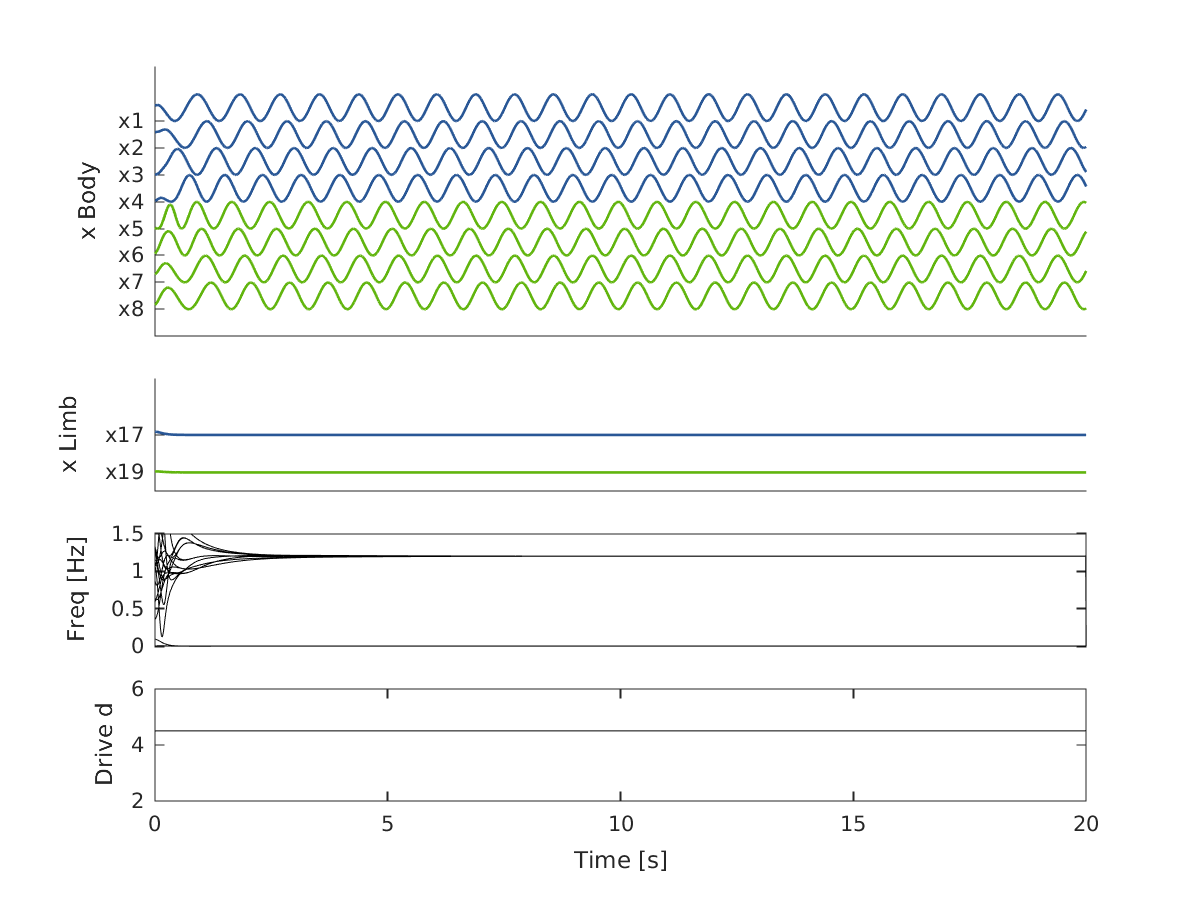
\includegraphics[width=0.5\textwidth]{fig/figure7a-swim.png}
	\caption{Simulation of the salamander CPG model for a duration of 20 seconds while applying a constant drive of 4.5 and resulting in a steady swimming behaviour.}
	\label{fig:7a-swim}
\end{figure}

\begin{figure}[!h]
	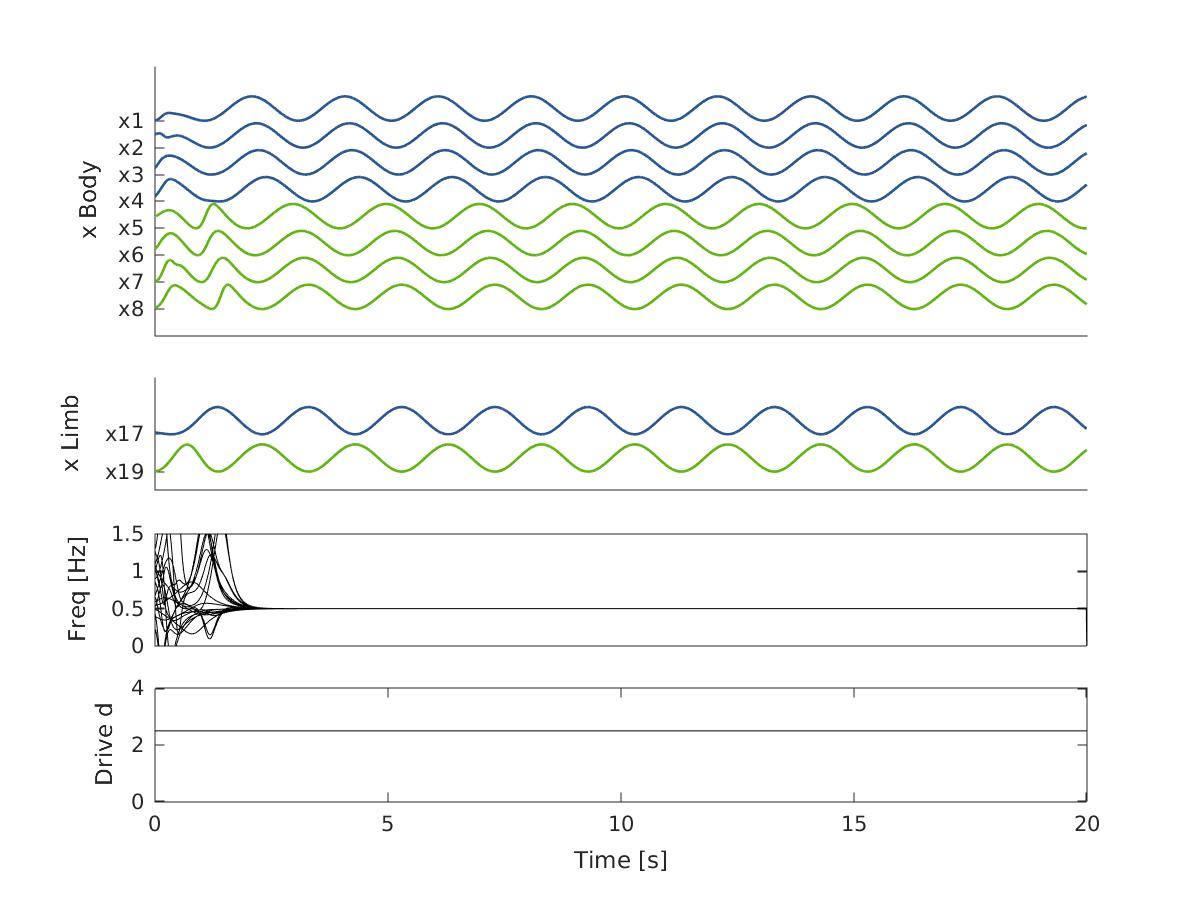
\includegraphics[width=0.5\textwidth]{fig/figure7a-walk.png}
	\caption{Simulation of the salamander CPG model for a duration of 20 seconds while applying a constant drive of 2.5 and resulting in a steady walking behaviour.}
	\label{fig:7a-walk}
\end{figure}

\begin{figure}[!h]
	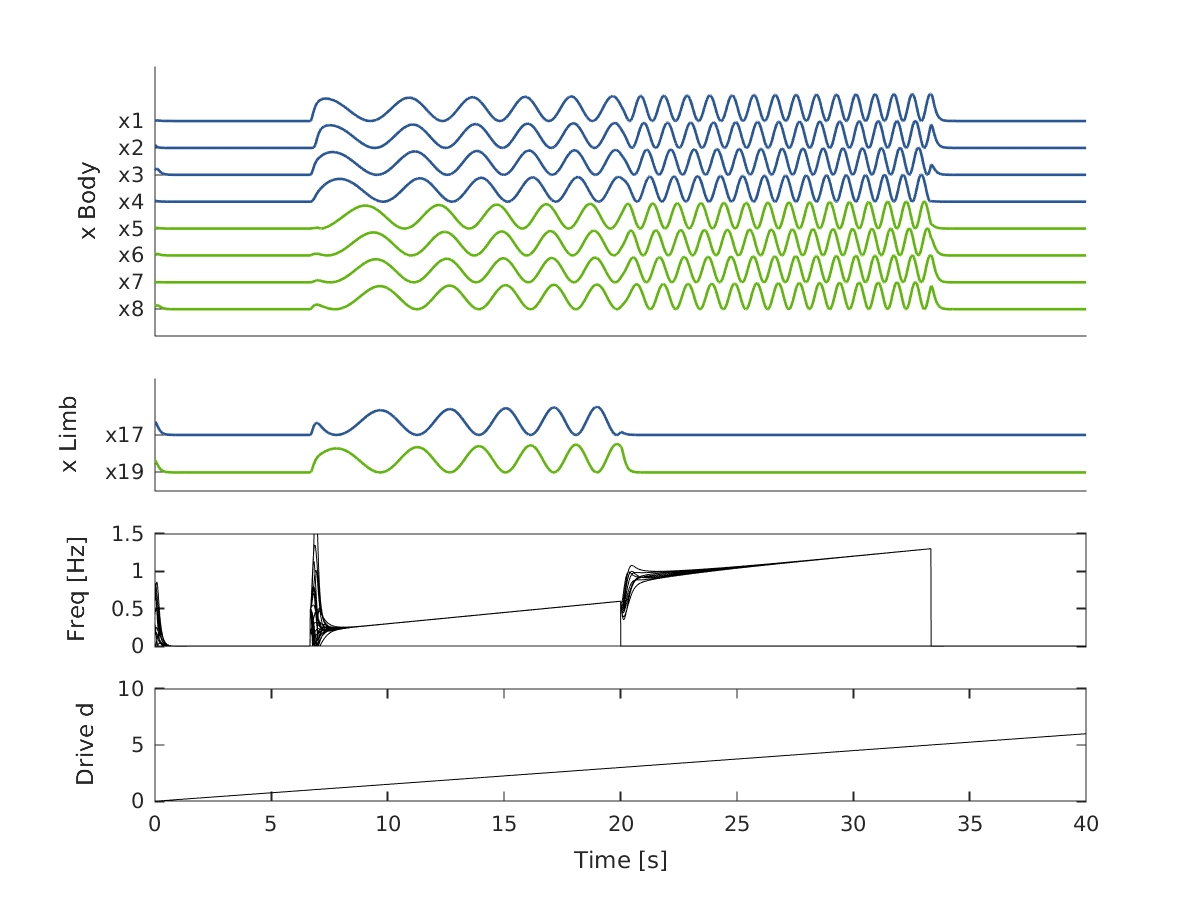
\includegraphics[width=0.5\textwidth]{fig/figure7a-drivegradient.png}
	\caption{Simulation of the salamander CPG model for a duration of 40 seconds while applying a linearly increasing drive from 0 to 6 and resulting in a transition from rest to walking to swimming and back to rest.}
	\label{fig:7a-transition}
\end{figure}

To analyse the transition from a walking to a swimming behaviour another simulation was run during which the model was subjected to a linearly increasing drive from 0 to 6 (see figure \ref{fig:7a-transition}). Up to around second 7 into the simulation, the CPG model stabilizes into resting mode, during which all limb and axial oscillators are inactive. Around 7 seconds into the simulation, the drive reaches a value of 1, which is the threshold value at which all oscillators have a non-zero intrinsic frequency (see figure \ref{fig:7a-saturation}), thus driving the system to oscillate. The system then starts off in a chaotic manner before stabilizing in a walking behaviour as previously described in figure \ref{fig:7a-walk}, but with linearly increasing frequency. Since the intrinsic frequencies of the oscillators and more importantly the limb oscillators has a linear dependence on the drive for values between 1 and 3, it is not surprising that the walking frequency increases with the linearly increasing drive. Once the drive reaches a value of 3 around 20 seconds into the simulation the walking behaviours suddenly stops before rapidly being replaced by a swimming behaviour. As seen before with the walking phase and because the intrinsic frequency of the axial oscillators is also linearly dependent on the drive, the swimming frequency also increases linearly for a while, although one should note that the axial oscillators had experienced a sudden jump in frequency once the limb oscillators were inactivated around the 20th second of simulation. This jump is due to the constant difference in intrinsic frequencies between limb and axial oscillators in the walking range of the drive between 1 and 3. In this range the axial oscillators have an intrinsic frequency about a quarter Hertz above the intrinsic frequency of the limb oscillators at any time, but are held down the limb frequency through a coupling strength as observed in figure \ref{fig:7a-walk}. Finally, around 33 seconds into the simulation, the drive reaches a value of 5, which is the threshold value above which the intrinsic frequency of the axial oscillators also goes to zero (see figure \ref{fig:7a-saturation}), which explains why the CPG model returns to a resting state at which all oscillators remain quite.

\begin{figure}[!h]
	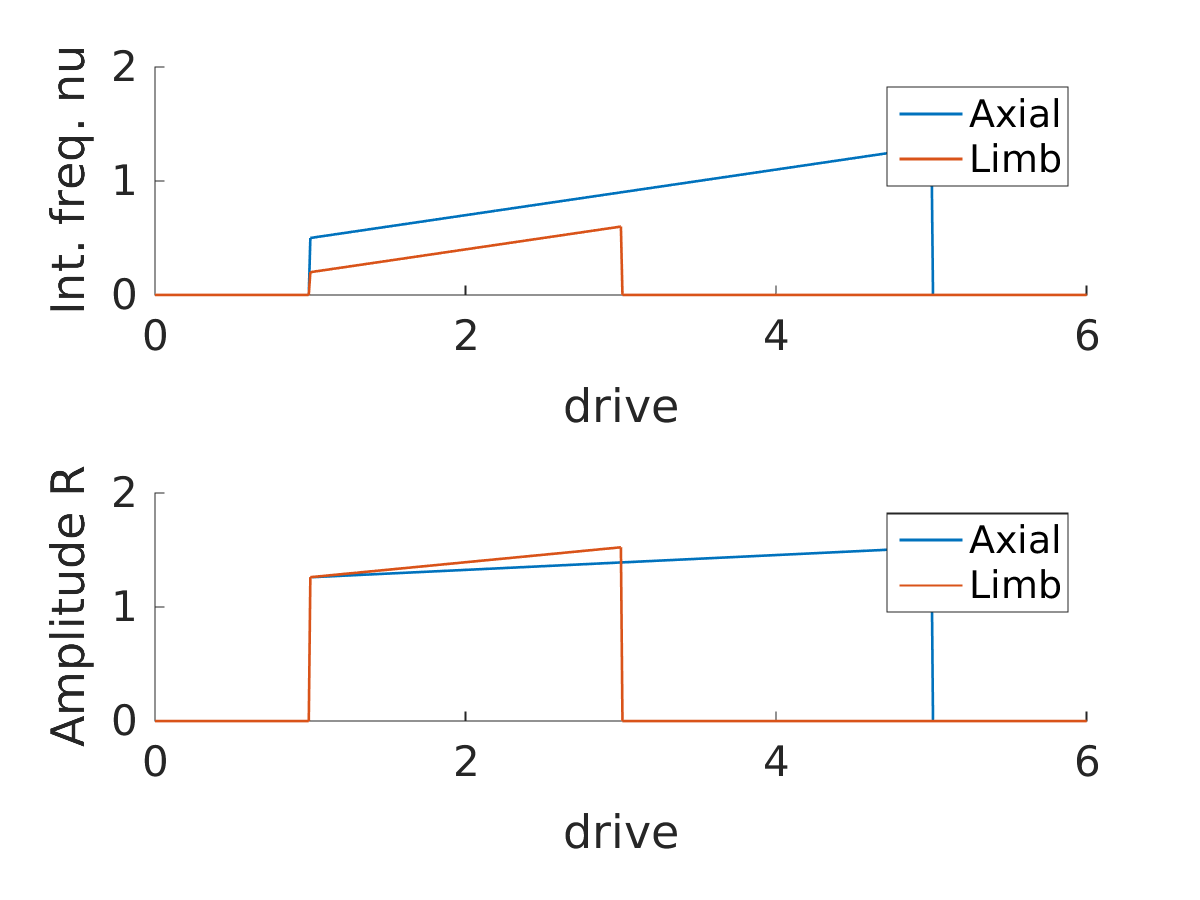
\includegraphics[width=0.5\textwidth]{fig/figure7a-frequency-drive-dependence.png}
	\caption{Plot of the frequency dependence of the intrinsic frequencies and amplitudes of axial and limb oscillators.}
	\label{fig:7a-saturation}
\end{figure}


\section{Handling of perturbations}
Natural systems, such as the salamander are constantly subjected to noise, both internal and external. The CPG model's robustness when faced to noise was therefore tested. First, the system was simulated when subjected to a noisy drive with linearly increasing noise variance in time (see figure \ref{fig:7b-drive}). This was performed using both an average drive of 2 and of 4 to compare the stability of the walking and the swimming behaviour to noise and both displayed a qualitatively similar dynamic. The oscillators maintained a clean oscillation up to a variance of 0.5, where they started to develop a visible high frequency noise. However the swimming and walking frequencies remain relatively intact up to a noise variance around 1, at which point the low frequency oscillations are more notably disturbed and start to slightly slow down. This behaviour intensifies until the main walking and swimming oscillation start to completely break down when subjected to noise of variance approximately 1.5 and the main frequencies have decreased by half. From there on the oscillators become more and more random, but one should note that they maintain a good correlation. Most noticeably for the swimming case, the phase gradient the axial oscillators is visible for the low frequency component at least up to a noise variance of 4 and despite the constant decrease in frequency of this synchronized oscillations. Furthermore the phase difference between the uppermost and lowest axial oscillator also seems to stay around $2\pi$ no matter what. 

\begin{figure}[!h]
	%\textbf{A}
    	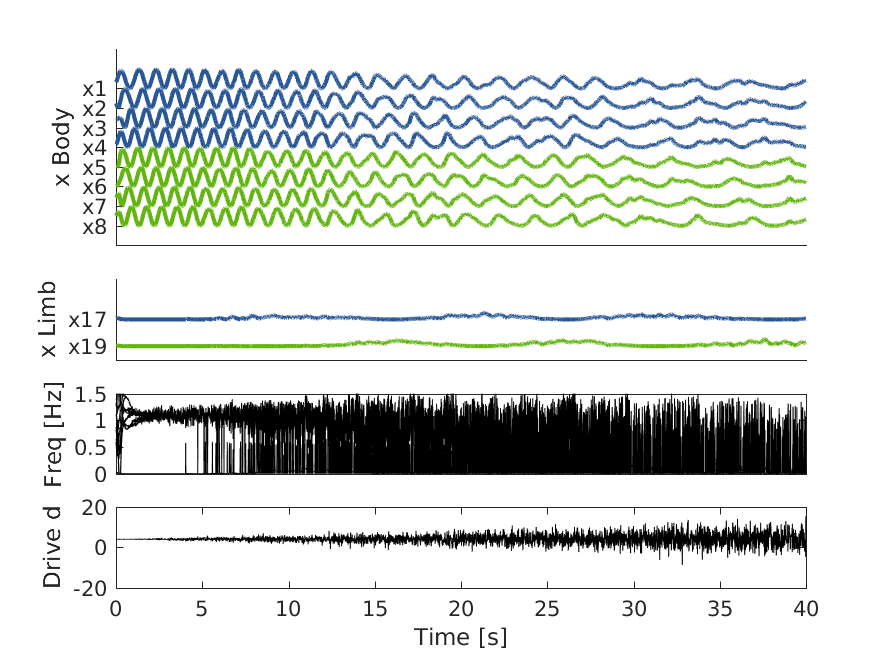
\includegraphics[width=0.5\textwidth]{fig/figure7b_drive-increasing-gaussian-swim.png}
    %\textbf{B}
	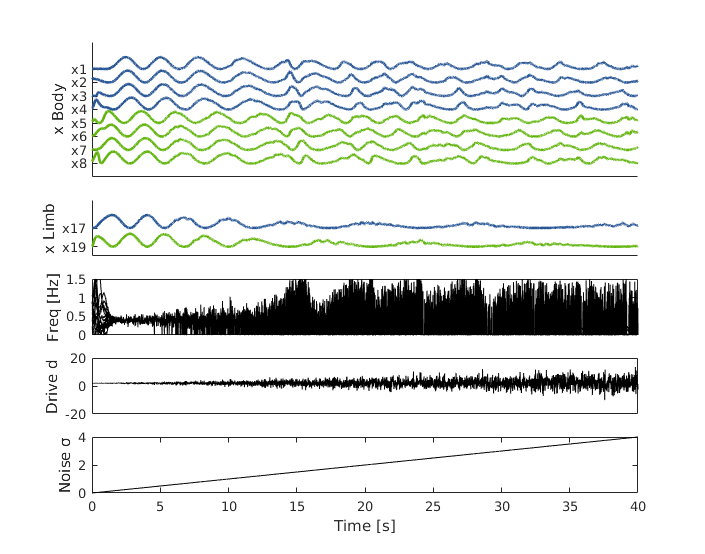
\includegraphics[width=0.5\textwidth]{fig/figure7b_drive-increasing-gaussian-walk.png}
	\caption{Simulations of the salamander CPG model with drive of constant mean, but linearly increasing noise variance from 0 to 4. Upper: Simulation in swimming mode with drive mean of 4. Lower: Simulation in swimming mode with drive mean of 2.}
	\label{fig:7b-drive}
\end{figure}

efsegfrgr fwer f
wef
wef
wfe 
ver
u
a
er
g
uiu
u
butini
ui
n
8
nk8
ki
9i
nkn9

k9
ni
t


\end{document}
